% Created 2020-12-10 Thu 10:26
% Intended LaTeX compiler: pdflatex
\documentclass[11pt]{article}
\usepackage[utf8]{inputenc}
\usepackage[T1]{fontenc}
\usepackage{graphicx}
\usepackage{grffile}
\usepackage{longtable}
\usepackage{wrapfig}
\usepackage{rotating}
\usepackage[normalem]{ulem}
\usepackage{amsmath}
\usepackage{textcomp}
\usepackage{amssymb}
\usepackage{capt-of}
\usepackage{hyperref}
\usepackage{amsthm}
\usepackage{url}
\usepackage[margin=1.25in]{geometry}
\usepackage{hyperref}
\usepackage[dvipsnames]{xcolor}
\usepackage{booktabs}
\usepackage{enumitem}
\usepackage{verbatim}
\usepackage[numbered,framed]{matlab-prettifier}
\lstset{
style              = Matlab-editor,
basicstyle         = \mlttfamily,
escapechar         = ",
mlshowsectionrules = true,
}
\usepackage{minted}
\newtheorem*{definition}{Definition}
\newtheorem*{example}{Example}
\newtheorem*{theorem}{Theorem}
\newtheorem*{corollary}{Corollary}
\newtheorem*{exercise}{Exercise}
\newtheorem*{problem}{Problem}
\newtheorem{question}{Question}
\newcommand{\gr}{\textcolor{ForestGreen}}
\newcommand{\rd}{\textcolor{red}}
\newcommand{\R}{\mathbb{R}}
\newcommand{\p}{\mathbb{P}}
\newcommand{\frall}{\ \forall}
\author{Chris Ackerman, Eketerina Gurkova, Ali Haider Ismail, Ben Pirie and Luna Shen}
\date{\today}
\title{Econ202A Homework \#2}
\hypersetup{
 pdfauthor={Chris Ackerman, Eketerina Gurkova, Ali Haider Ismail, Ben Pirie and Luna Shen},
 pdftitle={Econ202A Homework \#2},
 pdfkeywords={},
 pdfsubject={},
 pdfcreator={Emacs 28.0.50 (Org mode 9.3)}, 
 pdflang={English}}
\begin{document}

\maketitle
\newpage

\begin{enumerate}
\item In this economy, assume that $r = \delta$. Prove Hall’s Corollary 1 and 2, and 4. In addition, how would you go about estimating the implied regression in Corrolary 4?
Solving the constrained maximization problem we have the following
\begin{align*}
    \mathcal{L} = E_t \sum_{\tau=0}^{T-\tau} \frac{u(c_{t+\tau})}{(1+\delta)^\tau} + \lambda \left(\sum_{\tau=0}^{T-\tau} \frac{c_{t+\tau}}{(1+r)^\tau} - \sum_{\tau=0}^{T-\tau}\frac{w_{t+\tau}}{(1+r)^\tau} - A_t \right)
\end{align*}

The FOC with respect to $c_{t+\tau}$ is then given by
\begin{align*}
    [c_{t+\tau}]: \quad  E_t \frac{u'(c_{t+\tau})}{(1+\delta)^\tau} + \lambda \frac{1}{(1+r)^\tau} = 0
\end{align*}
\begin{align*}
    \tau = 0 & \Rightarrow E_t [u'(c_t)] = u'(c_t) = -\lambda\\
    \tau = 1 & \Rightarrow E_t [u'(c_{t+1})] = - \lambda \frac{1+\delta}{1+r}
\end{align*}

From this two conditions we get
\begin{align*}
    E_t [u'(c_{t+1})] =  \frac{1+\delta}{1+r} u'(c_t)
\end{align*}

\begin{corollary}
No information available in period $t$ apart from the level of consumption, $c_t$, helps predict future consumption, $c_{t+1}$, in the sense of affecting the expected value of marginal utility. In particular, income or wealth in periods $t$ or earlier are irrelevant, once $c_t$ is known. 
\end{corollary}

\begin{proof}
Once we obtain the equation above, we can conclude that both income or wealth do not predict the future level of consumption in the sense of affecting the expected value of marginal utility. Moreover, considering the case where $r=\delta$, we get
\begin{align*}
    E_t [u'(c_{t+1})] =   u'(c_t)
\end{align*}
which means that there are no other factors expect current level of consumption that affect the future consumption (assuming that we have time separable utility function, depending on consumption only).
\end{proof}

\begin{corollary}
Marginal utility obeys the regression relation, $u'(c_{t+1}) = \gamma u'(c_t) + \varepsilon_{t+1}$, where $\gamma = (1+\delta)/(1+r)$ and $\varepsilon_{t+1}$ is a true regression disturbance; that is, $E_t [\varepsilon_{t+1}] = 0$.
\end{corollary}

\begin{proof}
Taking the conditional expectation at period t we get
\begin{align*}
     E_t [u'(c_{t+1})] =  \gamma E_t [u'(c_t)] + E_t[\varepsilon_{t+1}]
\end{align*}
Since the consumption at period $t$ is known, $E_t [u'(c_t)] = u'(c_t)$. The relation from constrained maximization problem is that $E_t [u'(c_{t+1})] =  (1+\delta)/(1+r) u'(c_t)$. Then, indeed, the marginal utility can be expressed as the above stated regression relation with $\gamma = (1+\delta)/(1+r)$ and $E_t[\varepsilon_{t+1}] = E_t [u'(c_{t+1})] -  \gamma E_t [u'(c_t)] = E_t [u'(c_{t+1})] - (1+\delta)/(1+r) u'(c_t)=0$.
\end{proof}

\begin{corollary}[Corollary 4 from Hall's paper]
If the utility function has the constant elasticity of substitution form, $u(c_t) = c_t^{(\sigma-1)/\sigma}$, then the following statistical model describes the evolution of consumption: $c_{t+1}^{-1/\sigma} = \gamma c_t^{-1/\sigma} + \varepsilon_{t+1}$.
\end{corollary}

\begin{proof}
From Corollary 2 we have that the marginal utility of consumption can be represented as the following regression relation
\begin{align*}
    u'(c_{t+1}) = \gamma u'(c_t) + \varepsilon_{t+1}
\end{align*}
Calculating the marginal utility for the constant elasticity of substitution utility form we get
\begin{align*}
    \frac{\sigma-1}{\sigma} c_{t+1}^{-1/\sigma} = \gamma \frac{\sigma-1}{\sigma} c_t^{-1/\sigma} + \varepsilon_{t+1}
\end{align*}
Since $(\sigma-1)/\sigma$ is a constant, we can rewrite this regression as follows (without loss of generality)
\begin{align*}
    c_{t+1}^{-1/\sigma} = \gamma c_t^{-1/\sigma} + \varepsilon_{t+1}^*
\end{align*}
where $\varepsilon_{t+1}^* = \sigma/(\sigma-1) \varepsilon_{t+1}$, and therefore, $E_t[\varepsilon_{t+1}^*] = E_t[\sigma/(\sigma-1) \varepsilon_{t+1}] = \sigma/(\sigma-1) E_t[\varepsilon_{t+1}] = 0$.
\end{proof}

For estimating this regression we propose the log transformation
\begin{align*}
    \ln c_{t+1} = \mu + \gamma \ln c_t + \epsilon_{t+1}
\end{align*}
Then we can apply OLS method to estimate this regression, which is asymptotically equivalent to MLE estimator. In this case, the coefficient will be interpreted as a $\gamma$-percentage increase in future consumption in response to a 1-percentage increase in the current consumption.

\newpage
\item Explain the economic intuition for why the stochastic process for income is irrelevant in terms of being able to forecast future consumption. 

Considering stochastic process for income implies that the deviations from some stationary level are unexpected, thus they do not affect consumption (and are actually disturbance). All the expected deviations (change of trend) are incorporated in current consumption, and do not have any additional information that can help predict the future consumption.

\newpage
\item Explain the economic intuition why if $r < \delta$, then consumption evolves as a random walk with positive drift, in which there is a constant term in the regression that is negative. 

Having that marginal utility obeys a random walk apart from the trend, we can consider small deviations from the steady state consumption and expand the implicit equation for $c_{t+1}$ and $c_t$ in a Taylor series.
\begin{align*}
   E_t [u'(\Bar{c}) + u''(\Bar{c})(c_{t+1}-\Bar{c})] = \frac{1+\delta}{1+r} [u'(\Bar{c}) + u''(\Bar{c})(c_{t}-\Bar{c})]\\
\end{align*}
which can be rewritten as
\begin{align*}
    c_{t+1} = \left(\frac{1+\delta}{1+r} -1 \right) \left(\frac{u'(\Bar{c})}{u''(\Bar{c})}-\Bar{c}\right) + \frac{1+\delta}{1+r} c_t + \varepsilon_{t+1}
\end{align*}
Since $r<\delta$, we conclude that $(1+\delta)/(1+r)-1>0$. Also, we know that by assumption made in Hall's paper utility function is strictly concave, thus $u''(\Bar{c}) <0$ and $u'(\Bar{c})/u''(\Bar{c})-\Bar{c}<0$. Hence, this regression can be rewritten as follows
\begin{align*}
    c_{t+1} = \mu + \gamma c_t + \varepsilon_{t+1}
\end{align*}
which is a random walk with a positive drift $\gamma$ and negative constant $\mu$.

Intuitively, this result can be obtained from the fact that under the permanent income hypothesis individual chooses current consumption by estimating the future ability to consume. Thus, any information and changes in income at time $t$ are unexpected, and make changes in future consumption unpredictable. Also, since the interest rate is lower than the rate of subjective time preference, individuals prefer to consume now, and future consumption responds more than 1 for 1 to a change in current consumption.

\newpage
\item  Obtain quarterly real consumption (in chained dollars) from the U.S.
national income and product accounts from 1950 through 2019. Fit the following
regression:
\[
\ln(c_t) = \mu + \lambda \ln(c_{t-1}) + u_t
\]

Attached here is the code used to download and estimate this model.

\lstinputlisting[caption = {Testing the Life Cycle-Permanent Income Hypothesis}]{testLifeCycleHypothesis.m}

The relevant output from Matlab is copied below.
The first output comes from fitting testing the model fit of the AR(1) on the data.
\begin{lstlisting}[caption={Matlab output from AR(1) model on data}, label=lst:data-output]
    Effective Sample Size: 280
    Number of Estimated Parameters: 3
    LogLikelihood: 954.097
    AIC: -1902.19
    BIC: -1891.29

                  Value       StandardError    TStatistic      PValue   
                __________    _____________    __________    ___________

    Constant      0.020958      0.0056916        3.6822        0.0002312
    AR{1}          0.99846      0.0007193        1388.1                0
    Variance    6.4235e-05     2.7222e-06        23.597      4.1773e-123
\end{lstlisting}

Here is the output from testing to see if an AR(1) model fits the residual from the above model.
\begin{lstlisting}[caption={Matlab output from AR(1) model on residuals}, label=lst:resid-output]
    ARIMA(1,0,0) Model (Gaussian Distribution):

                  Value       StandardError    TStatistic      PValue   
                __________    _____________    __________    ___________

    Constant    6.1197e-05     0.00049822       0.12283          0.90224
    AR{1}         0.060598       0.034226        1.7705         0.076641
    Variance    6.4005e-05     2.8928e-06        22.125      1.8103e-108
\end{lstlisting}

\newpage
\item  Do you think that this is a reasonable statistical model of the log of
consumption? (Your answer to this question may include a discussion regarding
the value of the autoregressive coefficient, the R-square, and whether there is
autocorrelation in the $u_t$ residuals.)
\begin{figure}[htp]
\centering
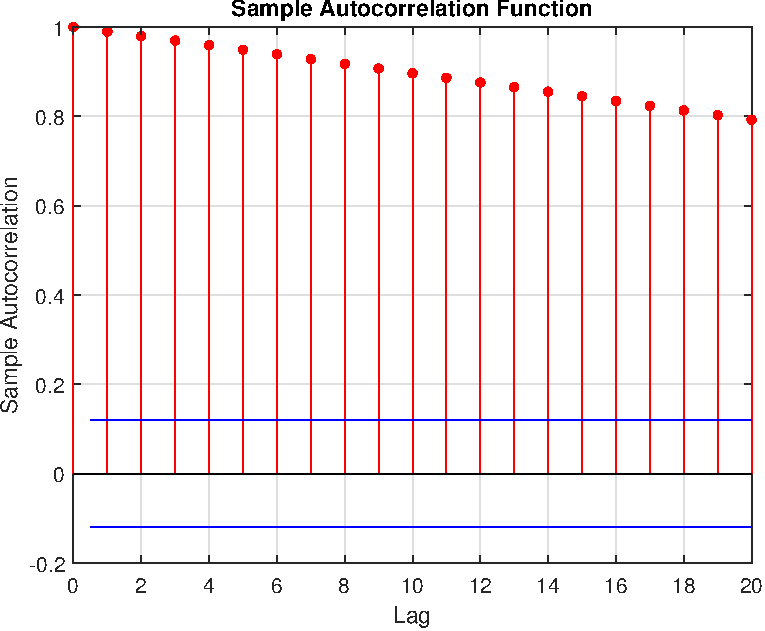
\includegraphics[scale=0.75]{data-autocorrelation-plot.pdf}
\caption{Question 4 - Autocorrelation plot of data}
\label{fig:q4-data-autocorrplot}
\end{figure}

\begin{figure}[htp]
\centering
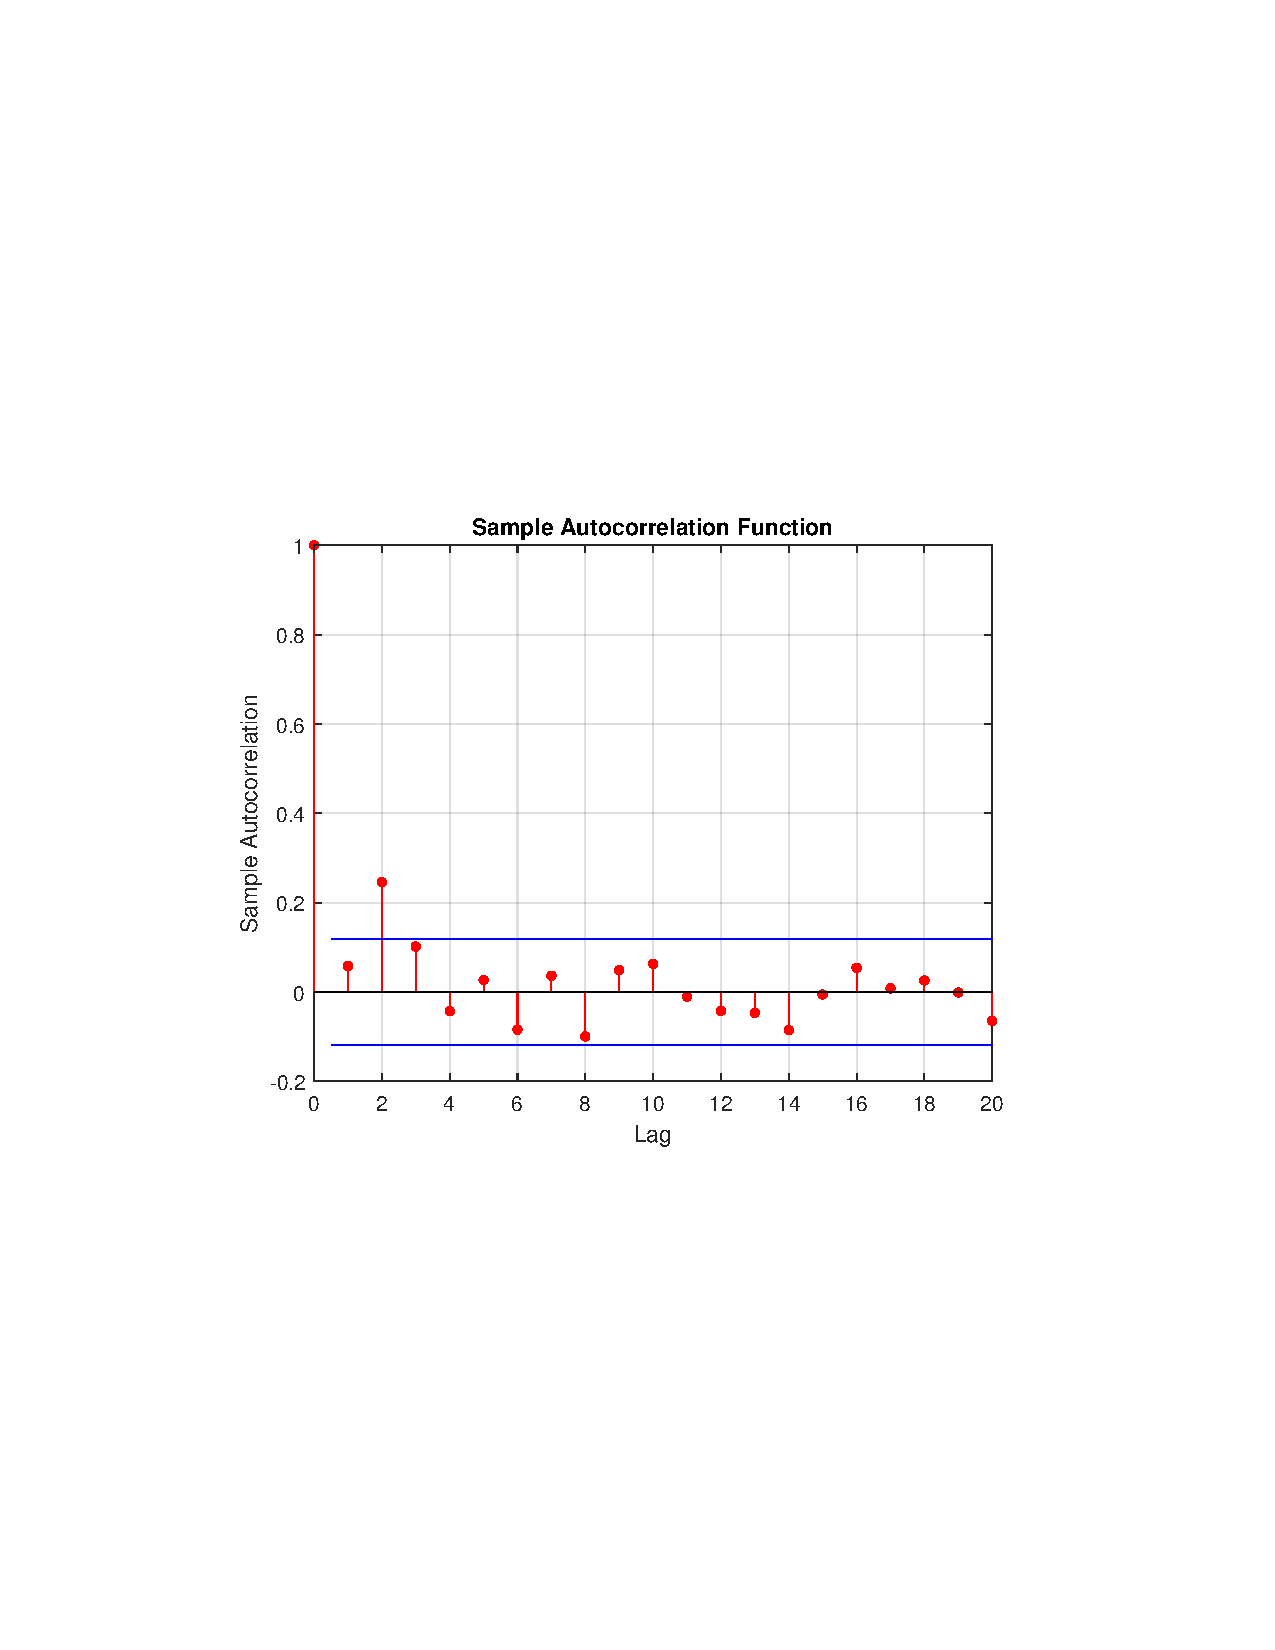
\includegraphics[scale=0.75]{residual-autocorrelation-plot.pdf}
\caption{Question 4 - Autocorrelation plot of residuals}
\label{fig:q4-residual-autocorrplot}
\end{figure}

\begin{figure}[htp]
\centering
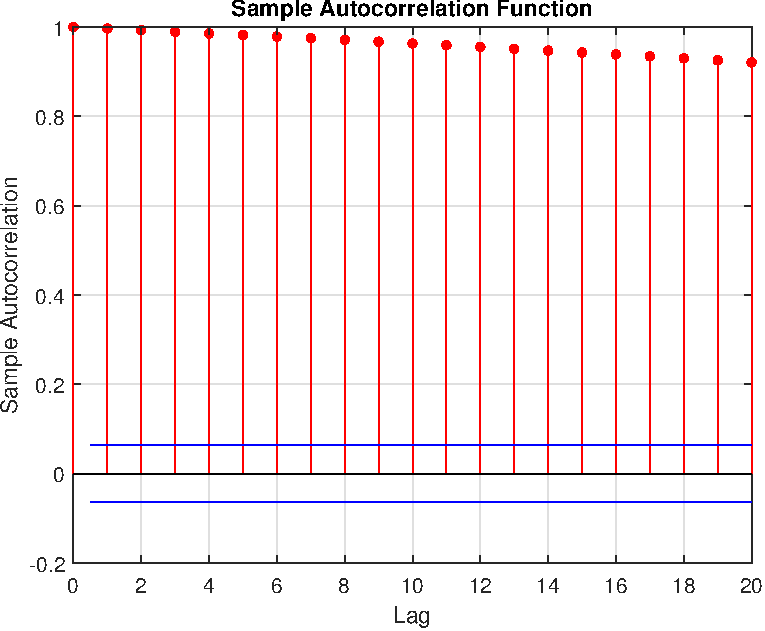
\includegraphics[scale=0.75]{data-simulated-autocorrelation-plot.pdf}
\caption{Question 4 - Autocorrelation plot of simulated data}
\label{fig:q4-data-simulated-autocorrplot}
\end{figure}

\begin{figure}[htp]
\centering
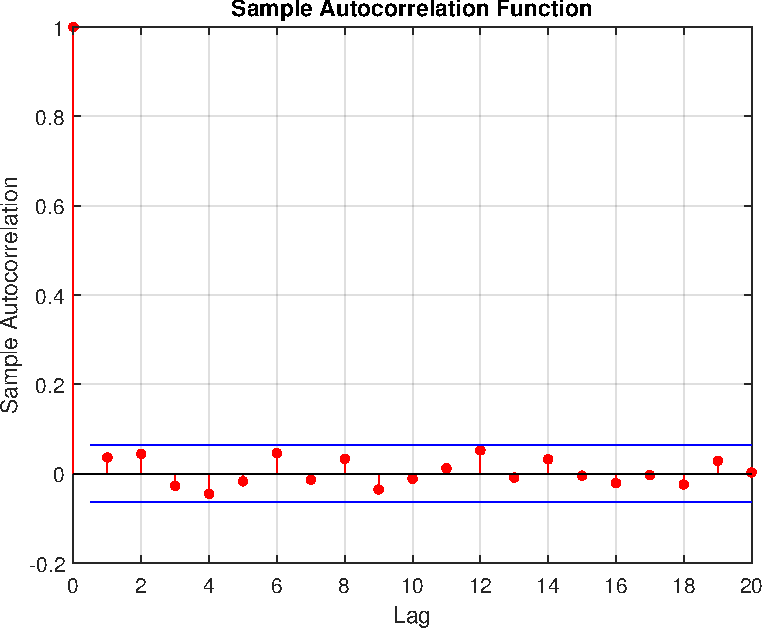
\includegraphics[scale=0.75]{residual-simulated-autocorrelation-plot.pdf}
\caption{Question 4 - Autocorrelation plot of simulated residuals}
\label{fig:q4-residual-simulated-autocorrplot}
\end{figure}

The model fits reasonably well. Firstly, the value of the value of the autoregressive coefficient in listing \ref{lst:data-output} (i.e the code output) is highly significant (with a p-value near 0 even), along with strong significance in the constant and variance. The R squared is \( 0.999857 \) (with the adjusted R being very similar since we are only estimating one lag) suggesting that the model explains the data very well. We also do a rudimentary test to see if the error is white noise in listing \ref{lst:resid-output} which shows that we cannot reject the null hypothesis at the 5\% significance that residuals have an AR(1) structure.

In figure \ref{fig:q4-data-autocorrplot} we see that the data clearly has a lagged structure. It is to be expected that with an AR(1) with a value for \( \rho \) close to 1, the lagged effects of the shock should be persistent. That is, we should {\itshape expect} non-zero auto correlation at all lags, which is in contrast to, say, an MA(q) process which only has non-zero autocorrelation for the first \( q \) lags. 

The autocorrelations of the residual of the above model are plotted in figure \ref{fig:q4-residual-autocorrplot}. This figure shows that most of the lags are within the confidence intervals around 0 and hence looks reasonably like white noise.

To verify our intuitions, we simulate an AR model with the same sample moments as the data in figures \ref{fig:q4-data-simulated-autocorrplot} and \ref{fig:q4-residual-simulated-autocorrplot}. Both confirm our findings that the data fits an AR(1) reasonably well.

There are some minor discrepancies when considering the Box-Ljuyng test that are persistent even with more lags. Despite that, we still believe that given the evidence that an AR(1) for consumption is a {\itshape reasonable} model.

\newpage
Next, consider the following economy.
\begin{align*}
\max & E_0 \sum^\infty_{t = 0}\beta^t \ln (c_t)\\
\intertext{subject to}
z_t A_t^{1 - \theta} k_t^\theta + (1 - \delta)k_t &= c_t + k_{t + 1}\\
A_t &= (1 + \gamma)^t, \quad t = 0, 1, \ldots \\
\ln(z_t) &= \rho \ln (z_{t - 1}) + \varepsilon_t,\quad \varepsilon_t \sim \mathcal{N}(0, \sigma^2_\varepsilon)
\end{align*}

Assume that the time period is annual. Construct a detrended version of
this economy and show the first order conditions. Choose $\beta$ so that the return
to capital in the steady state of the detrended economy is five percent, choose
$\theta$ so that capital’s share of income is 30 percent, and choose a depreciation rate
such that the share of investment to GDP in the steady state is 20 percent.
Choose $\rho = 0.95$, $\sigma^2_\varepsilon
 = .002$ and $\gamma = 0.02$.

\begin{align*}
\intertext{Rearranging terms, we have}
k_{t + 1} &= A_t^{1 - \theta} k_t^\theta + (1 - \delta) k_t - c_t\\
Y_t &= A_t^{1 - \theta} k_t^\theta\\
c_t &= (1 - \theta) A_t^{1 - \theta} k_t^\theta\\
\intertext{To detrend, divide by $A_t$. Let's define a few new variables,}
\hat{k}_t &= \frac{K_t}{A_t}\\
\hat{y}_t &= \frac{Y_t}{A_t}\\
\hat{c}_t &= \frac{C_t}{A_t}.\\
\intertext{Now, we can substitute these back into the original equations.}
A \hat{k}_{t + 1} &= \hat{y}_t + (1 - \delta) \hat{k}_t - \hat{c}_t\\
1 + \gamma \hat{k}_{t + 1} &= \hat{y}_t + (1 - \delta) \hat{k}_t - \hat{c}_t\\
\hat{y}_t &= k^\theta\\
\hat{c}_t &= (1 - \theta) \hat{y}_t.\\
\intertext{First order conditions give us}
\frac{1}{\hat{c}_t} &= \frac{\beta}{1 + \gamma} E_t \left\{\frac{1}{\hat{c}_{t + 1}}\left[\frac{\theta \hat{y}_{t + 1}}{\hat{k}_{t + 1}} + 1 - \delta \right]\right\}.\\
\intertext{In the steady state, we have}
\frac{\overline{c}}{\overline{y}} &= \frac{1 + \gamma - \beta(1 - \delta) - \theta \beta (1 + \gamma - 1 + \delta)}{1 + \gamma - \beta (1 - \delta)}.\tag{$\ast$}\label{consumption-share}\\
\intertext{Now let's solve for parameters. We're given $\gamma = 0.02$, and we have to figure out $\beta$, $\theta$ and $\delta$. Since we have Cobb Douglas production, $\theta = 0.3$. To solve for $\beta$, note that the 5\% return implies}
\beta &= \frac{1}{1.05}\\
&= 0.95238.\\
\intertext{To solve for $\delta$, we're going to use equation \ref{consumption-share}. We're told that investment in the steady state is 20\% of GDP, so that implies that consumption is 80\% of GDP,}
0.8 &= \frac{1.02 - 0.95238(1 - \delta) - 0.3 \cdot 0.95238 (1.02 - 1 + \delta)}{1.02 - 0.95238 (1 - \delta)}\\
\implies \delta &= .082.
\end{align*}

\newpage
\item 
 Log-linearize this model around its deterministic steady state. (For simplicity, assume that $z$ in the steady state is 1).

\begin{align*}
\text{Define } \tilde{x} &\equiv \log\left(\frac{\hat{x}}{\overline{x}}\right).\\
\intertext{From the Euler equation, we have}
\frac{\hat{c}_{t + 1}}{\hat{c}_t} &= \frac{\beta}{A} E_t [\theta z_{t + 1}\hat{K}^{\theta - 1}_{t + 1} + 1 - \delta].\\
\intertext{Substituting our log linearization into the left-hand side, we have}\\
\frac{\overline{c}\exp(\tilde{c}_{t + 1})}{\overline{c} \exp (\tilde{c}_t)} &\approx (1 + \tilde{c}_{t + 1})(1 - \tilde{c}_t)\tag{LHS}\\
&\approx 1 + \tilde{c}_{t + 1} - \tilde{c}_t \tag{LHS}.\\
\intertext{Doing the same thing on the right-hand side, we have}
\frac{\beta}{A} E_t [\theta \overline{z} (1 + \tilde{z}_{t + 1})\overline{K}(1 + (\theta - 1)\hat{K}_{t + 1}) + 1 - \delta] &=
\frac{\beta}{A} E_t [\theta \overline{z} \overline{K}^{\theta - 1}(\theta - 1)\tilde{K}_{t + 1} + \theta \overline{z} \overline{K}^{\theta - 1}\tilde{z}_{t + 1} + 1 - \delta]\\
\intertext{In the steady state,}
1 &= \frac{\beta}{A}(\theta \overline{z} \overline{K}^{\theta - 1} + 1 - \delta),\\
\overline{z} &= 1.\\
\intertext{We can use these to simplify the log-linearized Euler equation:} 
\tilde{c}_{t + 1} - \tilde{c}_t &= \frac{\beta}{A} E_t [\theta \overline{K}^{\theta - 1}(\theta - 1)\tilde{K}_{t + 1} + \theta \overline{K}^{\theta - 1} \tilde{z}_{t + 1}].\\
\intertext{Now, let's do the same thing to the budget constraint.}
\hat{c}_t + A\hat{K}_{t + 1} &= z_t \hat{K}_t^\theta + (1 - \delta)\hat{K}_t \\
\overline{c}(1 + \tilde{c}_t) + A \overline{K} (1 + \hat{K}_{t + 1}) &= \overline{c} + A\overline{K} + \overline{c}\tilde{c}_t + A\overline{K}\tilde{K}_{t + 1}\tag{LHS}\\
\overline{z}(1 + \tilde{z}_t)\overline{K}^\theta (1 + \theta \tilde{K}_t) + (1 - \delta)\overline{K}(1 + \tilde{K}_t) &=
\overline{z} \overline{K}^\theta + \overline{z} \overline{K}^\theta \theta \tilde{K}_t + \overline{z} \overline{K}^\theta \tilde{z}_t + (1 - \delta) \overline{K} + (1 - \delta)\overline{K} \tilde{K}_t \tag{RHS}.\\
\intertext{In the steady state,}
\overline{c} + A \overline{K} &= \overline{z}\overline{K}^\theta + (1 - \delta)\overline{K},\\
\overline{z} &=1,
\intertext{so we can simplify this expression to}
\overline{c}\tilde{c}_t + A\overline{K}\tilde{K}_{t + 1} &= \overline{K}^\theta \theta \tilde{K}_t + \overline{K}^\theta \tilde{z}_t + (1 - \delta)\overline{K}\tilde{K}_t,\\
\intertext{or}
\tilde{k}_{t + 1} &= \frac{\overline{K}^{\theta - 1}}{A} \theta \tilde{K}_t + \frac{\overline{K}^{\theta - 1}}{A} \tilde{z}_t + \frac{1 - \delta}{A}\hat{K}_t - \frac{\overline{c}}{A \overline{K}} \tilde{c}_t.\\
\intertext{Finally, for the stochastic process, }
\ln (z_t) &= \rho \ln (z_{t - 1}) + \varepsilon_t\\
\ln (\overline{z}\exp(\tilde{z}_t)) &= \rho \ln (\overline{z} \exp(\tilde{z}_{t - 1})) + \varepsilon_t\\
\ln (\overline{z}) + \tilde{z}_t &= \rho \ln (\overline{z}) + \rho \tilde{z}_{t - 1} + \varepsilon_t \\
\implies \tilde{z}_t &= \rho \tilde{z}_{t - 1},\\
\intertext{or}
\tilde{z}_{t + 1}&= \rho \tilde{z}_t.\\
\end{align*}
\begin{align*}
\intertext{Putting everything together, the log-linearized version of this economy is}
\tilde{c}_{t + 1} &= E_t \left\{\frac{\beta \theta \overline{K}^{\theta - 1}}{A}\left((\theta - 1)\left[\frac{\theta \overline{K}^{\theta - 1} + 1 - \delta}{A}\tilde{K}_t + \frac{\overline{K}^{\theta - 1}}{A}\tilde{z}_t - \frac{\overline{c}}{A \overline{K}} \tilde{c}_t\right] + \rho \tilde{z}_t \right) + \tilde{c}_t \right\}\\
\hat{k}_{t + 1} &= \frac{\theta \overline{K}^{\theta - 1} + 1 - \delta}{A} \hat{K}_t + \frac{\overline{K}^{\theta - 1}}{A} \tilde{z}_t - \frac{\overline{c}}{A \overline{K}}\tilde{c}_t\\
\tilde{z}_{t + 1} &= \rho \tilde{z}_t.
\end{align*}

\newpage
\item Use the formula of Blanchard and Kahn to show that there is a unique
stationary solution to the linearized system.

\lstinputlisting[caption = {Using BK to show there is a unique stationary solution}]{question_7.m}

\newpage
\item Using a random number generator (Matlab has a built-in function for
this), draw 1100 values of $\varepsilon$ to construct the $z$ process. Using these values of $z$,
and assuming that $k_0$ is equal to its steady state value, use the linearized system
to construct 1100 values values of output, consumption, and investment.
\\ The answer to this problem is written in Python.
\inputminted[linenos]{python}{q8.py}

\begin{figure}[htp]
\begin{center}
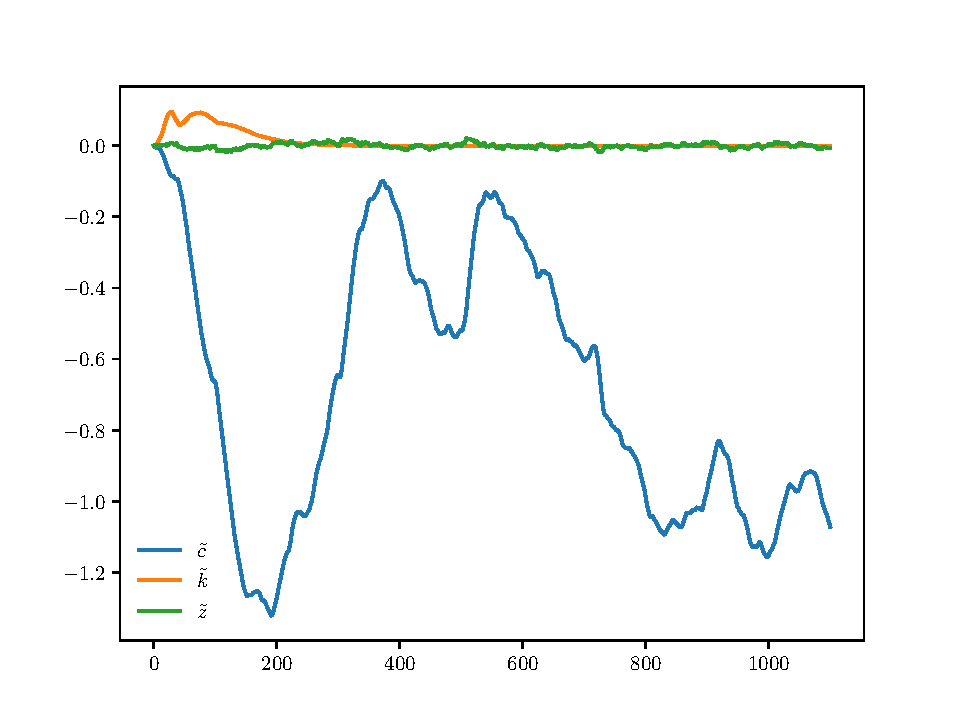
\includegraphics[scale=0.75]{log-linear-simulations.pdf}
\caption{Simulated log deviations}
\end{center}
\end{figure}

\begin{figure}[htp]
\begin{center}
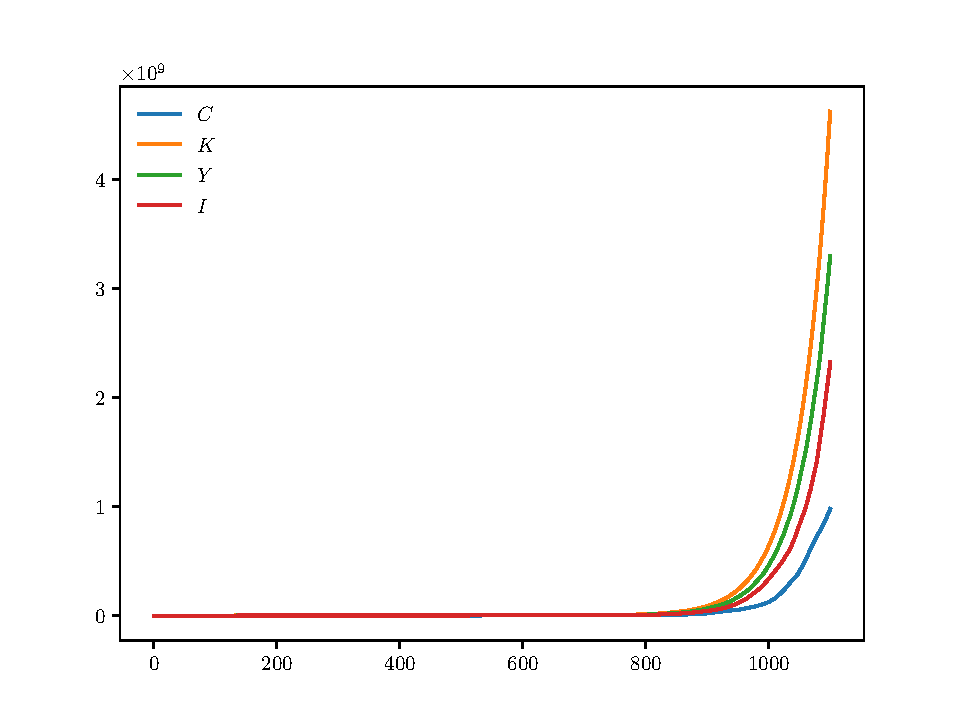
\includegraphics[scale=0.75]{my-economy-simulations.pdf}
\caption{Simulated Consumption, Investment, Output, and Capital}
\end{center}
\end{figure}


\newpage
\item Discard the first 100 observations, and then fit an AR(1) process to the
log of consumption, measured as the log-deviation of consumption from the
steady state value. Report the value of the AR(1) coefficient in the regression,
and evaluate whether there is autocorrelation in the residuals.

\lstinputlisting[caption = {Fitting AR(1) to Simulated Data}]{MacroHW2_Q9.m}

\begin{center}
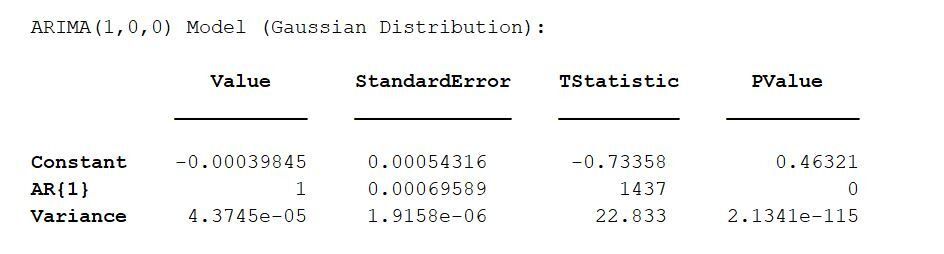
\includegraphics[scale=0.75]{MacroHW2_Q9.JPG}
\end{center}

\begin{figure}[htp]
\centering
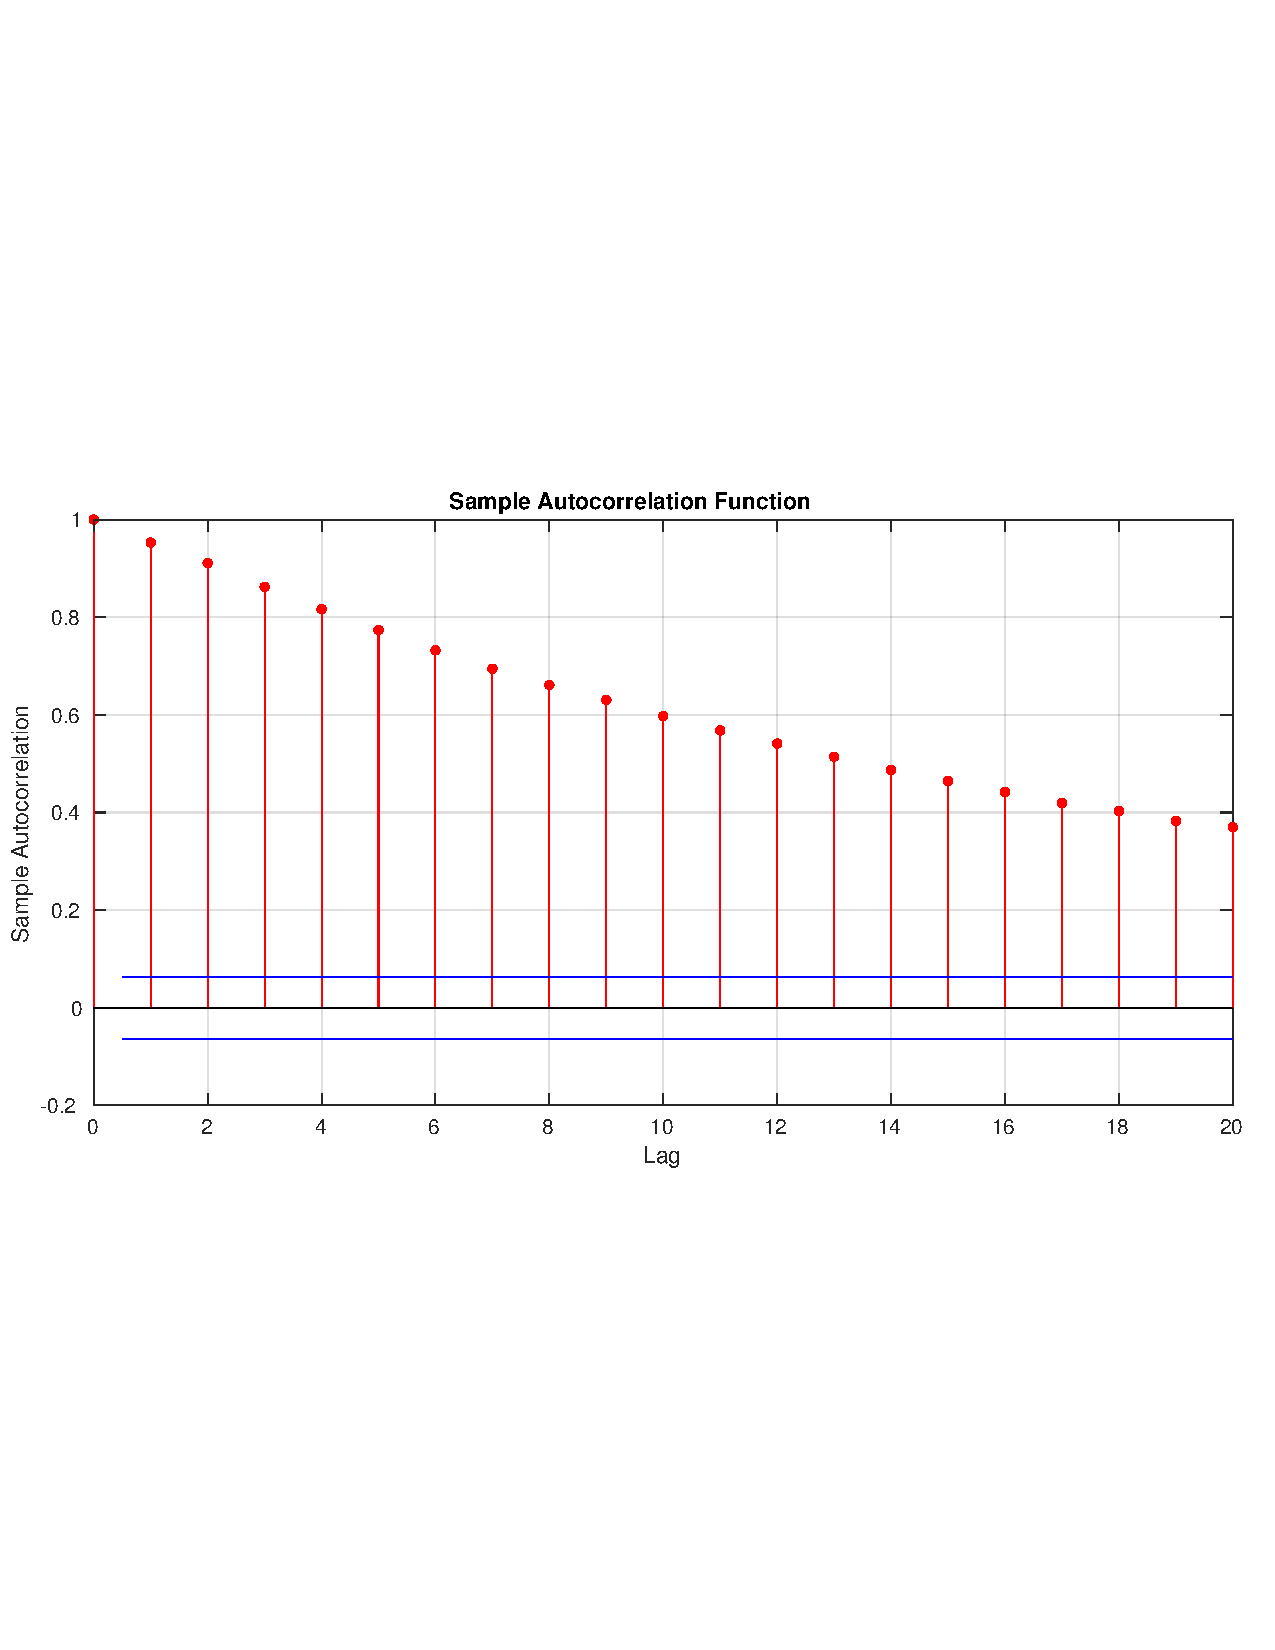
\includegraphics[scale=0.75]{Q9_ResidualAutocorrelationPlot.pdf}
\caption{Question 9 - Residual Autocorrelation}
\end{figure}

\newpage
\item Compare the regression coefficient in (9) and your assessment of the
autocorrelation in the residuals, to your answers in (4) and (5). Does the RBC
model provide a good approximation to consumption dynamics? What does it
tell us about using consumption data to try to discriminate between the Hall
\end{enumerate}
\end{document}